\begin{figure}[ht]
  \centering
  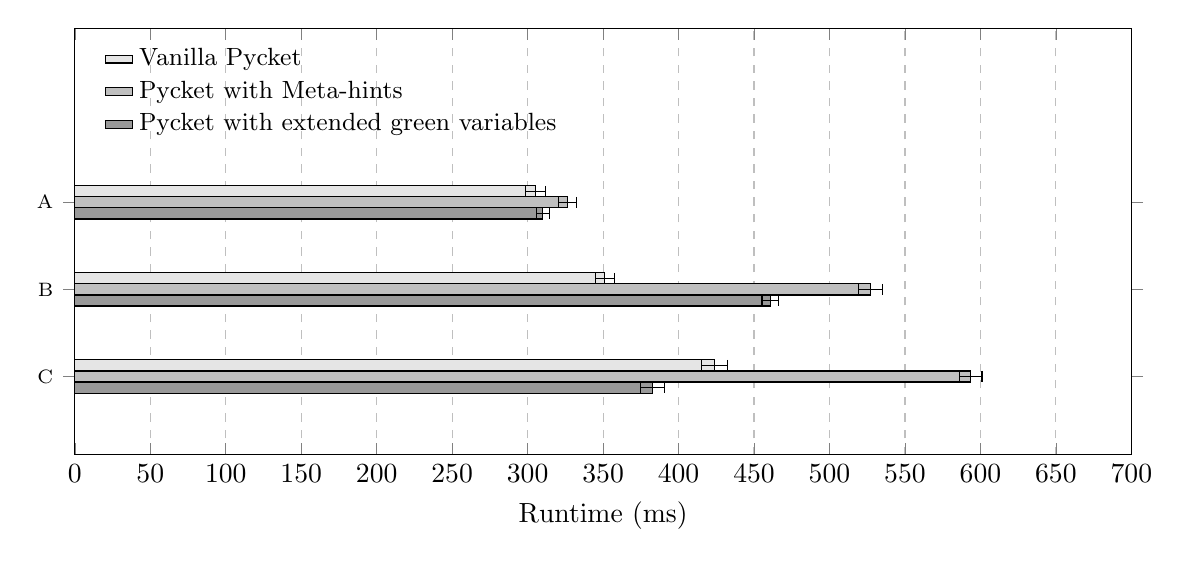
\begin{tikzpicture}
  \begin{axis}[
    xbar,
    width=15cm,
    height=7cm,
    xlabel={Runtime (ms)},
    ytick={1,2,3},
    yticklabels={C, B, A},
    yticklabel style={font=\scriptsize},
    xmin=0,
    xmax=700,
    ymin=0.1, ymax=5,
    xmajorgrids=true,
    grid style=dashed,
    clip=false,
    legend style={
        at={(0.02,0.98)},
        anchor=north west,
        draw=none,
        fill=none,
        legend cell align=left,
        font=\small,
        legend columns=1,
    },
    legend image code/.code={
        \draw[#1,fill] (0cm,-0.05cm) rectangle (0.35cm,0.05cm);
    },
    error bars/x dir=both,
    error bars/x explicit,
  ]
% Vanilla Pycket
\addplot[
  fill=gray!20,
  draw=black,
  bar width=4pt,
  bar shift=4pt,
  error bars/x dir=both,
  error bars/x explicit,
] coordinates {
  (305.25,3) +- (6.43,0)   % shalloww
  (351.2,2) +- (6.1,0)   % deep
  (423.9,1) +- (8.7,0) % random
};
% Pycket with Meta‑hints
\addplot[
  fill=gray!50,
  draw=black,
  bar width=4pt,
  bar shift=0pt,
  error bars/x dir=both,
  error bars/x explicit,
] coordinates {
  (326.3,3)  +- (5.8,0)   % shalloww
  (527.1,2)  +- (7.9,0)   % deep
  (593.7,1)  +- (7.3,0)  % random
};
% Pycket with extended green variables
\addplot[
  fill=gray!80,
  draw=black,
  bar width=4pt,
  bar shift=-4pt,
  error bars/x dir=both,
  error bars/x explicit,
] coordinates {
  (310.1,3)  +- (4.1,0)   % shalloww
  (460.7,2)  +- (5.4,0)   % deep
  (382.6,1)  +- (7.8,0)  % random
};
  \legend{Vanilla Pycket, Pycket with Meta-hints, Pycket with extended green variables}
  \end{axis}
  \end{tikzpicture}
  \caption{Experiment results of regular expression matching with targeted improvement approaches. All interpreters use the regexp linklet. Lower is better.}
  \label{fig:approaches-regexp-experiment}
\end{figure}
